% 3. The relevant data exploration process (pre-processing, feature extraction/selection,
% clustering and visualization)


\section{Data exploration process}

\subsection{Pre-processing}
\subsubsection{Treatment of missing values}
Our dataset do not have missing values, so there is no need to treat them.
\subsubsection{Treatment of anomalous values}
\red{Quizá hay que quitar algunas personas por ser demasiado jóvenes comparadas con el resto}
\subsubsection{Treatment of incoherent values}
The variable FEV1 which is the Forced Expiratory Volume in 1 second, shows a few anomalously high values. Depending on factors lika age and sex of a patient the average value of the FEV1 is around 3-6 litres, whereas the dataset shows values up to 86. As most of the values are within 0 and 10 we assume that the dataset contains the FEV1 in litres. To decide which values are to be determined as outliers we calculate the FEV1/FVC ratio which gives the percentage of the lung volume exhaled in the first second over the whole exhaled volume. All patients having a unrealistic ratio higher than 100\%, which are 22 patients, are determined to be outliers and eliminated. We chose not to apply any stricter constraints because the dataset does not include the sex of the patients which influences the normal values of the FEV1 much.

Source of knowledge about FEV1 and FVC:
https://www.nuvoair.com/blogs/blog/do-you-know-how-to-interpret-the-results-of-your-spirometry-test

\todo[inline]{Redactar que FEV1 está mal, referenciar algún artículo que hable
sobre el tema y para justificar que está mal, decidir qué haremos con esos pacientes (eliminarlos, o inferir
sus valores de FEV1 en función de sus vecinos) y si los inferimos poner el proceso
como lo hemos hecho}
\red{El FEV1 tiene valores incoherentes. La mayoría están sobre 3, pero algunos
están sobre 60}
\begin{figure}[bh]
\centering
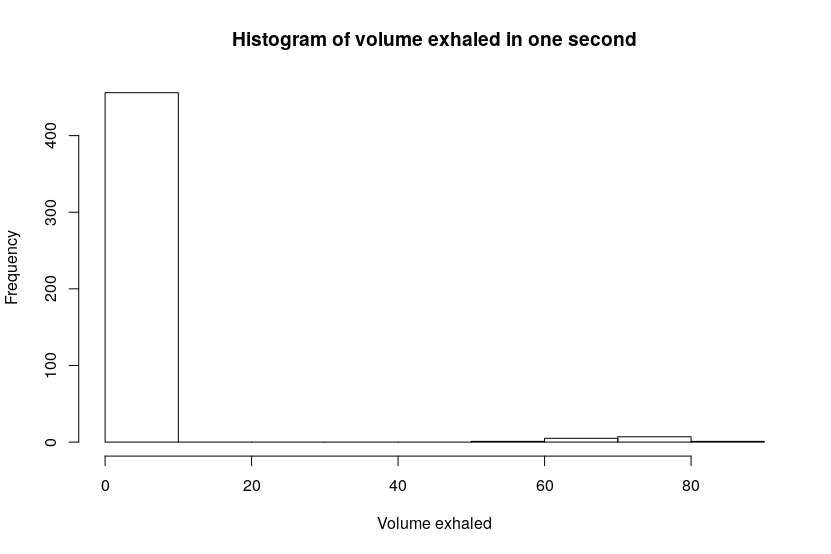
\includegraphics[width=10cm]{histFEV1}
\label{fig:histFEV1}
\caption{Show the ammount of people having each value}
\end{figure}
\subsubsection{Coding of non-continuous or non-ordered variables}
% \todo[inline]{El código que convierta nuestras variables categóricas en tiras
% de 0s y 1s}
\subsubsection{Possible elimination of irrelevant variables}

Some of the variables of our dataset are not well represented. In particular:

\begin{center}
\begin{tabular}{|c|c|}
  \hline
  \textbf{DGN} & There is just one patient with DGN = 1 and just 8 have DGN = 8 \\
  \hline
  \textbf{PAD} & Just 8 patients have PAD = True \\
  \hline
  \textbf{ASHTMA} & Just 2 patients have ASHTMA = True \\
  \hline
\end{tabular}
\end{center}

\todo[inline]{Redactar bien esta parte, indicando que puesto que tenemos pocos
datos, podemos permitirnos hacer varias ejecuciones, y que probaremos cada
combinación de eliminar y no eliminar cada una de estas variables y veremos
cual da mejores resultados con la cross-validation}

%
% \red{Algunas variables están muy poco representadas:}
% \red{Haremos los experimentos dos veces, uno con todos los datos originales,
% y otro quitando el atributo de MI, ASHTMA, DGN1 y DGN8, y entonces veremos cual
% da mejores resultados}
% \begin{itemize}
%   \item DGN: Solo un paciente tiene DGN1, y solo 2 tienen DGN8
%   \item Solo 2 pacientes tienen MI == True
%   \item Solo 8 pacientes tienen PAD == True
%   \item Solo 2 pacientes tienen ASHTMA == True
% \end{itemize}
\subsubsection{Creation of new useful variables (Feature extraction)}
\red{Entender cómo funciona MCA, y ver si podemos sacar una variable nueva}
\red{Quizá es interesante añadir la variable FEV/FEV1}
\subsubsection{Normalization of the variables}
We need to normalize only our numeric variables, which are the AGE, FEV and FV1.


\red{Solo se pueden normalizar FVC, FEV1 y AGE. Miraremos cuales dan mejores
resultados}
\subsubsection{Transformation of the variables}
Acording to \red{the paper we found} the accetable range for skewness in a numeric
variable is $(-2, +2)$. The skewness of our original variables AGE, FVC and FEV are:

\begin{center}
\begin{tabular}{| c | c |}
  \hline
  AGE & -0.1899413 \\
  FVC & 0.5417132 \\
  FEV1 & 5.597584 \\
  \hline
\end{tabular}
\end{center}

But we have to take into account that we've eliminated \red{22} patients, so the
new values are:

\todo[inline]{Poner los nuevos valores}

As the three variables are in the specified range, there is no need of
transforming them.

% \red{Skewness es la asimetría de los datos respecto a la media.}
% \red{Como la mayoría de nuestras variables son categóricas, no tiene mucho
% sentido medir el skewness, ni tampoco corregirlo}
% \red{Kurtosis igual que el skewness, no es necesario porque la mayoría con
% categóricas}
 % consultar si debemos ignorar este punto
% \todo[inline]{El código en r para corregir la asimetría (skewness) de los datos}
% \red{Es aceptable un skewness entre -2 y +2. AGE y FVC ya están en este rango, por
% lo tanto no hay que hacer nada con ellos. FEV1 sí que se sale, pero los datos que
% tiene son erroneos. Por lo tanto los transformatemos de alguna forma (eliminarlos
% o inferirlos) y miraremos el skewness de esos nuevos datos. (suponemos que entonces
% sí que estarán en ese rango, y por tanto no habrá que aplicar la transformación)}

\red{Referenciar (y leer un poco...) el paper}


%https://www.researchgate.net/publication/281345819_The_Research_Methods_Knowledge_Base


% \subsection{Feature extraction/selection}
\subsection{Clustering}
\red{hacer varios k-means con distintos valores de k (2,3,4,5,6) para ver si descubrimos algún cluster que nos permita crear una variable nueva}
\subsection{Visualization}
\red{Hacer MCA  }
